\renewcommand{\thechapter}{\arabic{chapter}}
\setcounter{chapter}{8}

\chapter{Approche multimodale}
\label{chap:chapter_8}
\chapterintro
Les travaux de la précédente partie ont porté sur le diagnostic de données malignes sur la modalité de \acrlong{rcm}, plus particulièrement de pathologies de \acrlong{lm} et de \acrlong{lmm}. Au premier niveau hiérarchique, soit celui des images, ces chapitres ont permis la mise en avant de méthodes de séparation des tissus sain, bénin et malin. Au second niveau hiérarchique, soit celui des lésions, ces méthodes permettent la prédiction des pathologies bénignes et malignes.\par

Ce nouveau chapitre rempli l'objectif de ce manuscrit en intégrant une dimension multimodale au processus de prise de décision. Tout d'abord, les aspects d'extraction de caractéristiques et de diagnostic par le biais de modèles de prédiction est traité pour chacune des modalités présentes dans le jeu de données utilisé. De plus, la calibration de ces modèles de prédiction est envisagée afin de rendre cohérent les décisions entre chacun d’entre eux. Puis, les systèmes multimodaux envisagés dans ce travail sont présentés selon deux axes~: une première méthode qualifiée comme sans mémoire, puis une seconde méthode qualifiée sous le terme d’avec mémoire. Finalement, les résultats obtenus à l'aide de ces méthodes sont présentés et discutés.\par
\newpage

\section{Méthodologie}
\section{Diagnostic des modalités}
\subsection{Diagnostic sur photographie clinique}
\subsection{Diagnostic sur dermatoscopie}
\subsection{Diagnostic sur microscopie confocale}
\clearpage

\section{Calibration de modèles}
La majeure partie des modèles de classification mettent à disposition des scores représentant l'appartenance à chacune des classes de la problématique visée. Ces scores sont à l'origine des prédictions de ces modèles et peuvent être obtenus de manière complémentaire à la prédiction. Ainsi, la classe n'est bien souvent que la manifestation de la classe ayant achevé le score le plus élevé.\par

Malheureusement, ces scores n'ont de sens que dans le contexte dans lequel ils ont été obtenus et ne conviennent pas lorsque plusieurs sources d'information différentes sont combinées. Ainsi, une estimation précise de la \textbf{probabilité} d'appartenance à chacune des classes est un indicateur plus pertinent dans ce type de stituation, ayant un sens en dehors du champ d'action propre à chacun de ces modèles~\cite{Zadrozny2002}.\par

Diverses méthodes sont proposées afin de transformer ces scores en probabilités, tout d'abord sur des problématiques binaires, puis plus tardivement sur des problématiques à classes multiples. Ce principe de transformation des scores en probabilités porte le nom de processus de \textbf{calibration}.\par

Ainsi, les méthodes de la littérature sont multiples
Isotonic regression, \cite{Zadrozny2002}
Bayesian Binning into Quantiles (BBQ) calibration\cite{Naeini2015}
Beta calibration,\cite{Kull2017}
Sigmoid,\cite{kull2017b}

\section{Système multimodal}
\subsection{Système séquentiel sans mémoire}
\subsection{Système séquentiel avec mémoire}

\section{Présentation des résultats}
\subsection{Protocole d’expérimentation}
\subsection{Résultats des expérimentation}

% Sequential - Pondéré
\begin{table}[H]
    \begin{tabular}{llllll}
        \toprule 
        Type                    & Modalité                          & Seuil             & Sans                  & Isotonic              & Sigmoid               \\ \midrule
        \multirow{4}{*}{Simple} & \multirow{2}{*}{Croissant}        & Croissant         & 0.72$\pm$0.14         & 0.65$\pm$0.14         & 0.66$\pm$0.10         \\ \cline{3-6}
                                &                                   & Décroissant       & 0.72$\pm$0.14         & 0.64$\pm$0.12         & 0.65$\pm$0.09         \\ \cline{2-6}
                                & \multirow{2}{*}{Décroissant}      & Croissant         & \textbf{0.81$\pm$0.08}& 0.61$\pm$0.11         & 0.79$\pm$0.10         \\ \cline{3-6}
                                &                                   & Décroissant       & 0.81$\pm$0.11         & 0.60$\pm$0.13         & 0.79$\pm$0.10         \\ \cline{1-6}
        \multirow{4}{*}{Double} & \multirow{2}{*}{Croissant}        & Croissant         & 0.71$\pm$0.09         & 0.64$\pm$0.18         & 0.71$\pm$0.13         \\ \cline{3-6}
                                &                                   & Décroissant       & 0.71$\pm$0.09         & 0.63$\pm$0.17         & 0.70$\pm$0.14         \\ \cline{2-6}
                                & \multirow{2}{*}{Décroissant}      & Croissant         & 0.77$\pm$0.13         & 0.71$\pm$0.16         & 0.77$\pm$0.12         \\ \cline{3-6}
                                &                                   & Décroissant       & 0.77$\pm$0.13         & 0.68$\pm$0.14         & 0.77$\pm$0.12         \\ \bottomrule
    \end{tabular}
\end{table}

% Sequential - Malignant
\begin{table}[H]
    \begin{tabular}{llllll}
        \toprule 
        Type                    & Modalité                          & Seuil             & Sans                  & Isotonic              & Sigmoid               \\ \midrule
        \multirow{4}{*}{Simple} & \multirow{2}{*}{Croissant}        & Croissant         & 0.79$\pm$0.10         & 0.76$\pm$0.09         & 0.79$\pm$0.07         \\ \cline{3-6}
                                &                                   & Décroissant       & 0.79$\pm$0.10         & 0.76$\pm$0.09         & 0.79$\pm$0.07         \\ \cline{2-6}
                                & \multirow{2}{*}{Décroissant}      & Croissant         & 0.85$\pm$0.11         & 0.74$\pm$0.07         & 0.85$\pm$0.10         \\ \cline{3-6}
                                &                                   & Décroissant       & 0.85$\pm$0.10         & 0.75$\pm$0.08         & \textbf{0.85$\pm$0.08}\\ \cline{1-6}
        \multirow{4}{*}{Double} & \multirow{2}{*}{Croissant}        & Croissant         & 0.80$\pm$0.07         & 0.77$\pm$0.11         & 0.78$\pm$0.10         \\ \cline{3-6}
                                &                                   & Décroissant       & 0.80$\pm$0.07         & 0.76$\pm$0.11         & 0.79$\pm$0.09         \\ \cline{2-6}
                                & \multirow{2}{*}{Décroissant}      & Croissant         & 0.83$\pm$0.11         & 0.80$\pm$0.11         & 0.83$\pm$0.09         \\ \cline{3-6}
                                &                                   & Décroissant       & 0.83$\pm$0.10         & 0.79$\pm$0.11         & 0.84$\pm$0.09         \\ \bottomrule    
    \end{tabular}
\end{table}


% Cumulative - Pondéré
\begin{table}[H]
    \begin{tabular}{llllll}
        \toprule 
        Type                    & Modalité                          & Seuil             & Sans                  & Isotonic              & Sigmoid               \\ \midrule
        \multirow{4}{*}{Simple} & \multirow{2}{*}{Croissant}        & Croissant         & 0.74$\pm$0.08         & 0.72$\pm$0.13         & 0.72$\pm$0.12         \\ \cline{3-6}
                                &                                   & Décroissant       & 0.72$\pm$0.09         & 0.74$\pm$0.14         & 0.70$\pm$0.13         \\ \cline{2-6}
                                & \multirow{2}{*}{Décroissant}      & Croissant         & 0.83$\pm$0.10         & 0.82$\pm$0.08         & 0.82$\pm$0.09         \\ \cline{3-6}
                                &                                   & Décroissant       & 0.82$\pm$0.10         & 0.81$\pm$0.08         & 0.80$\pm$0.12         \\ \cline{1-6}
        \multirow{4}{*}{Double} & \multirow{2}{*}{Croissant}        & Croissant         & 0.69$\pm$0.11         & 0.73$\pm$0.14         & 0.68$\pm$0.11         \\ \cline{3-6}
                                &                                   & Décroissant       & 0.68$\pm$0.12         & 0.72$\pm$0.12         & 0.68$\pm$0.13         \\ \cline{2-6}
                                & \multirow{2}{*}{Décroissant}      & Croissant         & \textbf{0.83$\pm$0.08}& 0.82$\pm$0.08         & 0.78$\pm$0.11         \\ \cline{3-6}
                                &                                   & Décroissant       & 0.82$\pm$0.08         & 0.81$\pm$0.08         & 0.78$\pm$0.12         \\ \bottomrule
    \end{tabular}
\end{table}

% Cumulative - Malignant
\begin{table}[H]
    \begin{tabular}{llllll}
        \toprule 
        Type                    & Modalité                          & Seuil             & Sans                  & Isotonic              & Sigmoid               \\ \midrule
        \multirow{4}{*}{Simple} & \multirow{2}{*}{Croissant}        & Croissant         & 0.82$\pm$0.06         & 0.81$\pm$0.09         & 0.81$\pm$0.09         \\ \cline{3-6}
                                &                                   & Décroissant       & 0.80$\pm$0.06         & 0.82$\pm$0.09         & 0.80$\pm$0.09         \\ \cline{2-6}
                                & \multirow{2}{*}{Décroissant}      & Croissant         & \textbf{0.87$\pm$0.06}& 0.86$\pm$0.06         & 0.85$\pm$0.08         \\ \cline{3-6}
                                &                                   & Décroissant       & 0.86$\pm$0.07         & 0.85$\pm$0.06         & 0.84$\pm$0.08         \\ \cline{1-6}
        \multirow{4}{*}{Double} & \multirow{2}{*}{Croissant}        & Croissant         & 0.79$\pm$0.08         & 0.81$\pm$0.10         & 0.78$\pm$0.08         \\ \cline{3-6}
                                &                                   & Décroissant       & 0.79$\pm$0.08         & 0.81$\pm$0.08         & 0.78$\pm$0.09         \\ \cline{2-6}
                                & \multirow{2}{*}{Décroissant}      & Croissant         & 0.86$\pm$0.06         & 0.86$\pm$0.06         & 0.83$\pm$0.09         \\ \cline{3-6}
                                &                                   & Décroissant       & 0.86$\pm$0.07         & 0.86$\pm$0.06         & 0.82$\pm$0.09         \\ \bottomrule
    \end{tabular}
\end{table}

\begin{figure}[H]
    \centering
    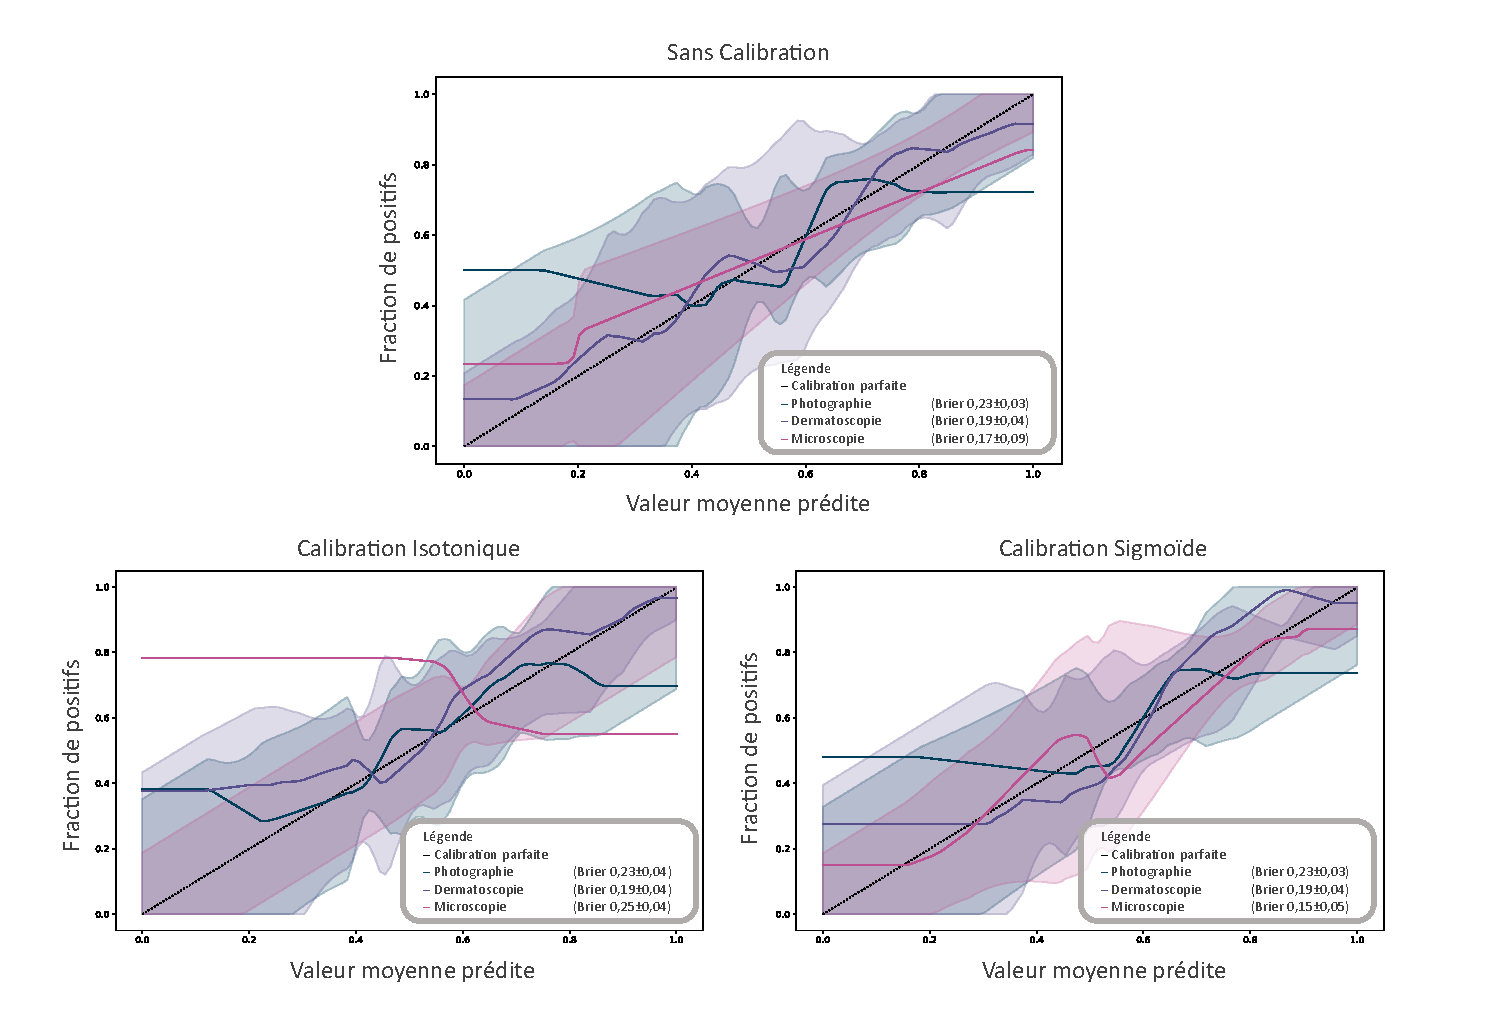
\includegraphics[width=\linewidth]{contents/chapter_8/resources/results_calibration_sequential.pdf}
    \caption{}
    \label{fig:results_calibration_sequential}
\end{figure}\par

\begin{figure}[H]
    \centering
    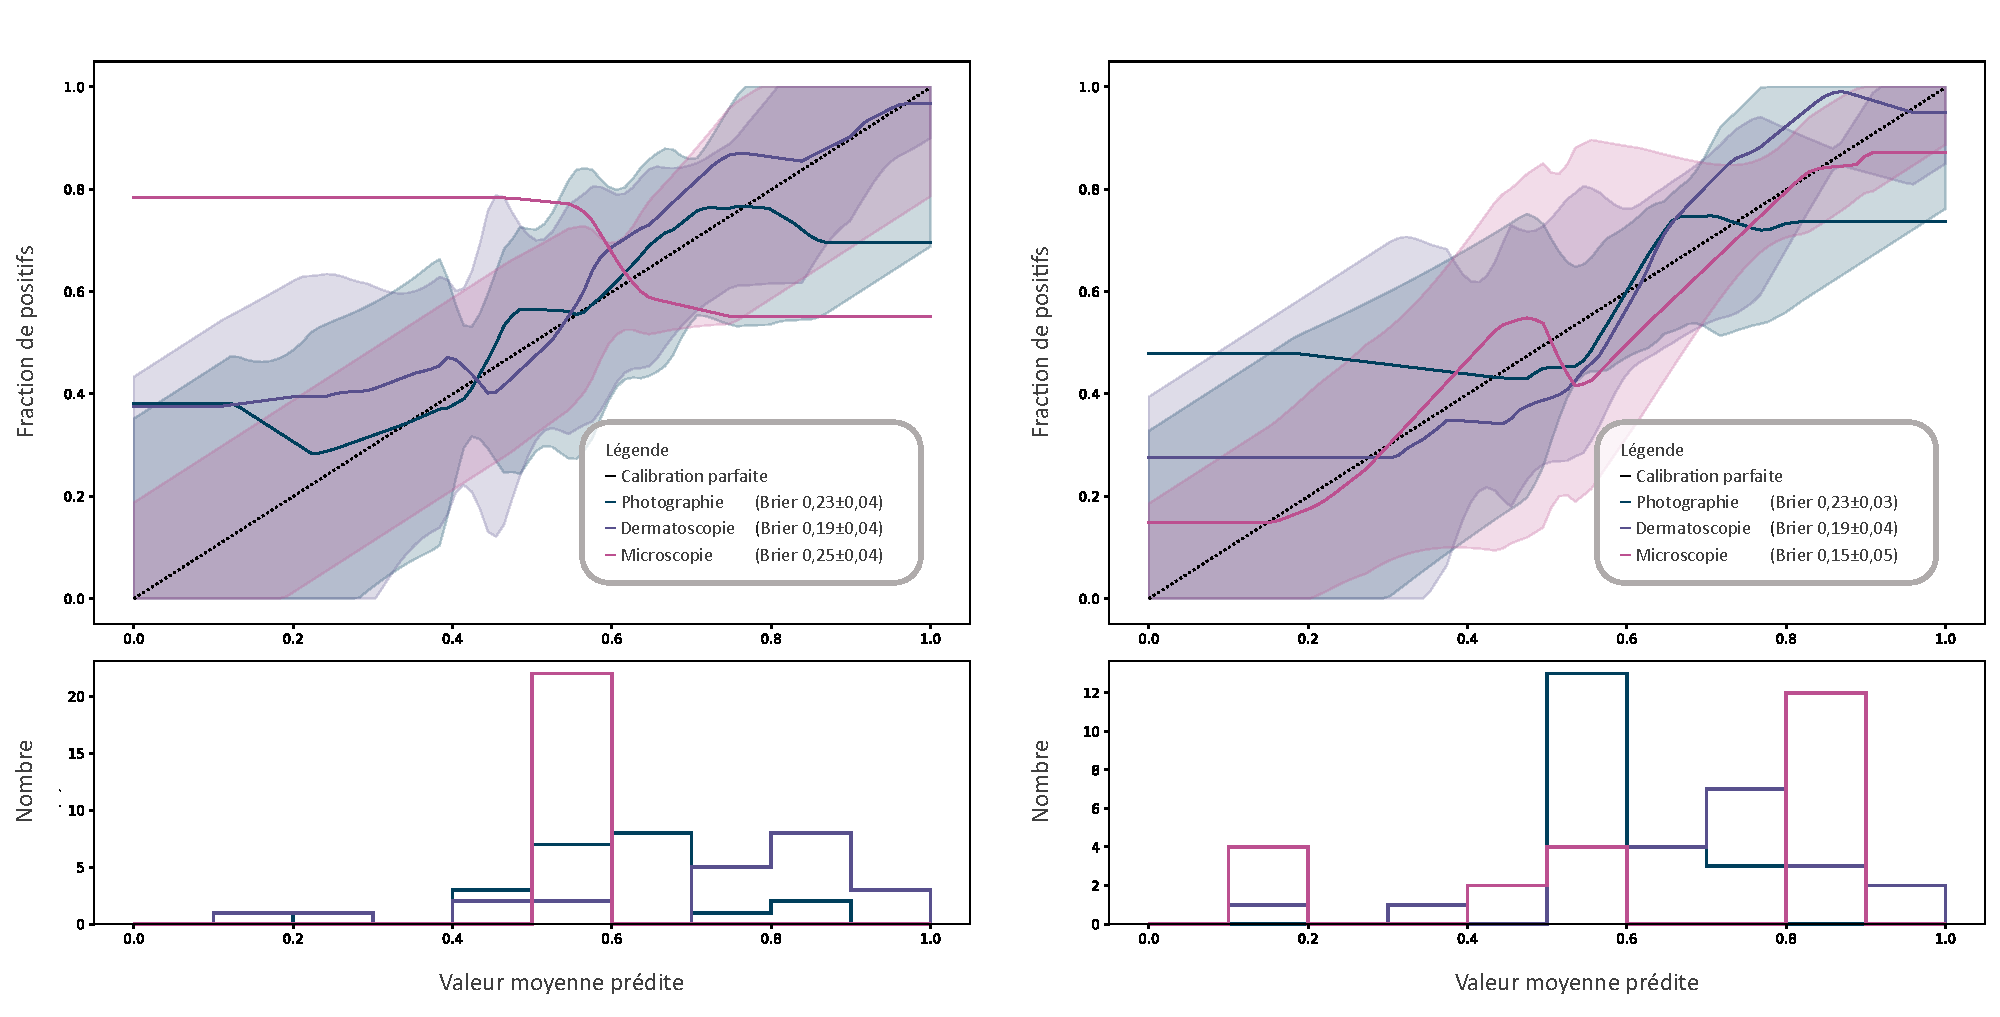
\includegraphics[width=\linewidth]{contents/chapter_8/resources/results_calibration_sequential_calibrated.pdf}
    \caption{}
    \label{fig:results_calibration_sequential_calibrated}
\end{figure}\par

\begin{figure}[H]
    \centering
    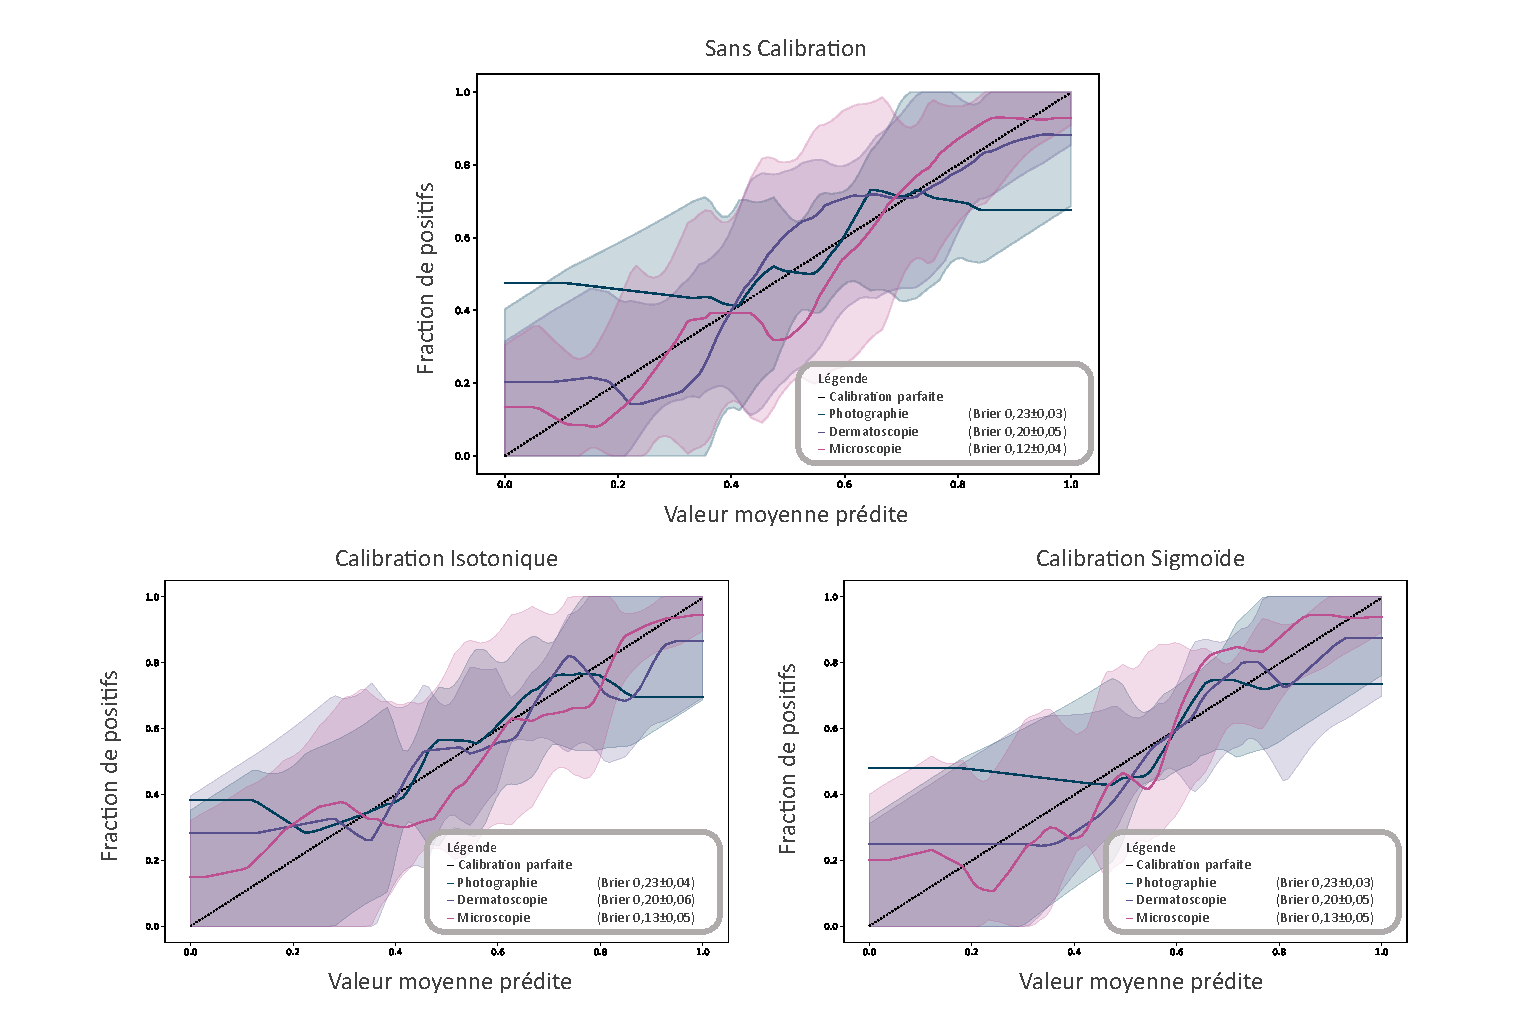
\includegraphics[width=\linewidth]{contents/chapter_8/resources/results_calibration_cumulative.pdf}
    \caption{}
    \label{fig:results_calibration_cumulative}
\end{figure}\par

\begin{figure}[H]
    \centering
    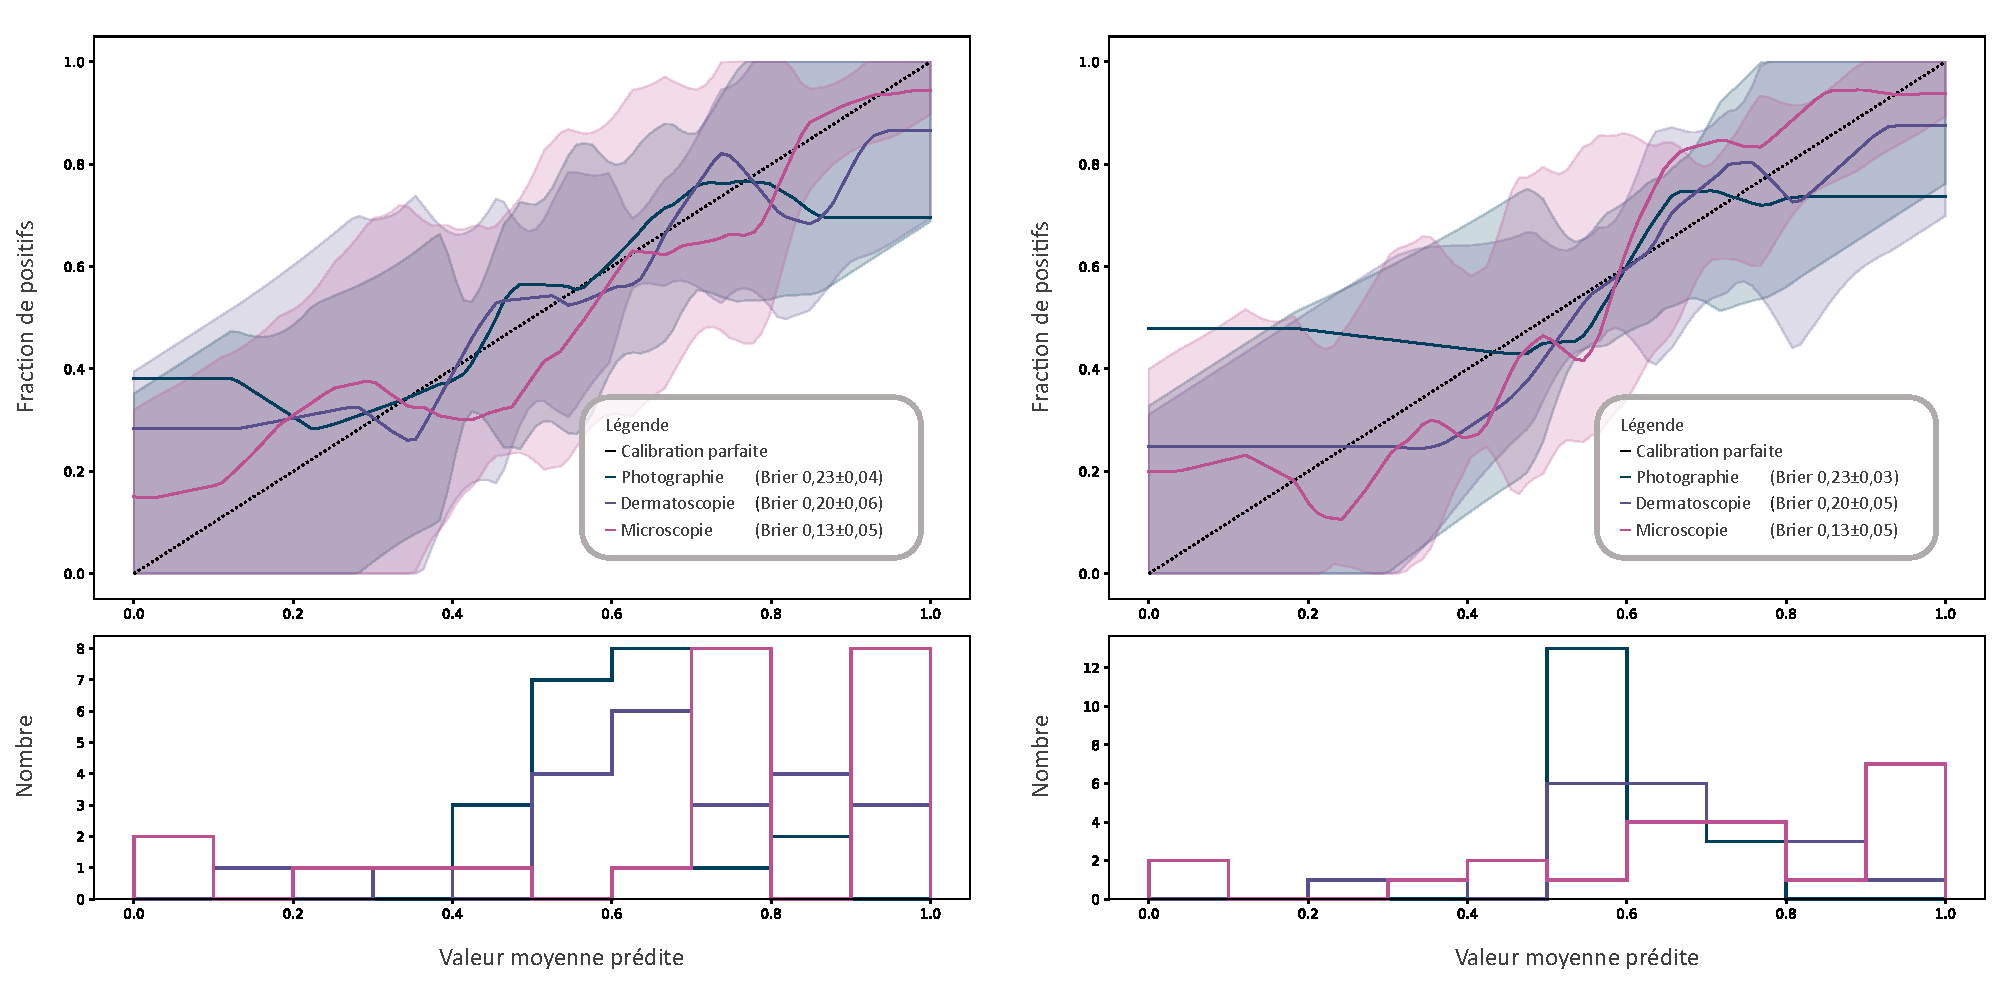
\includegraphics[width=\linewidth]{contents/chapter_8/resources/results_calibration_cumulative_calibrated.pdf}
    \caption{}
    \label{fig:results_calibration_cumulative_calibrated}
\end{figure}\par

\begin{figure}[H]
    \centering
    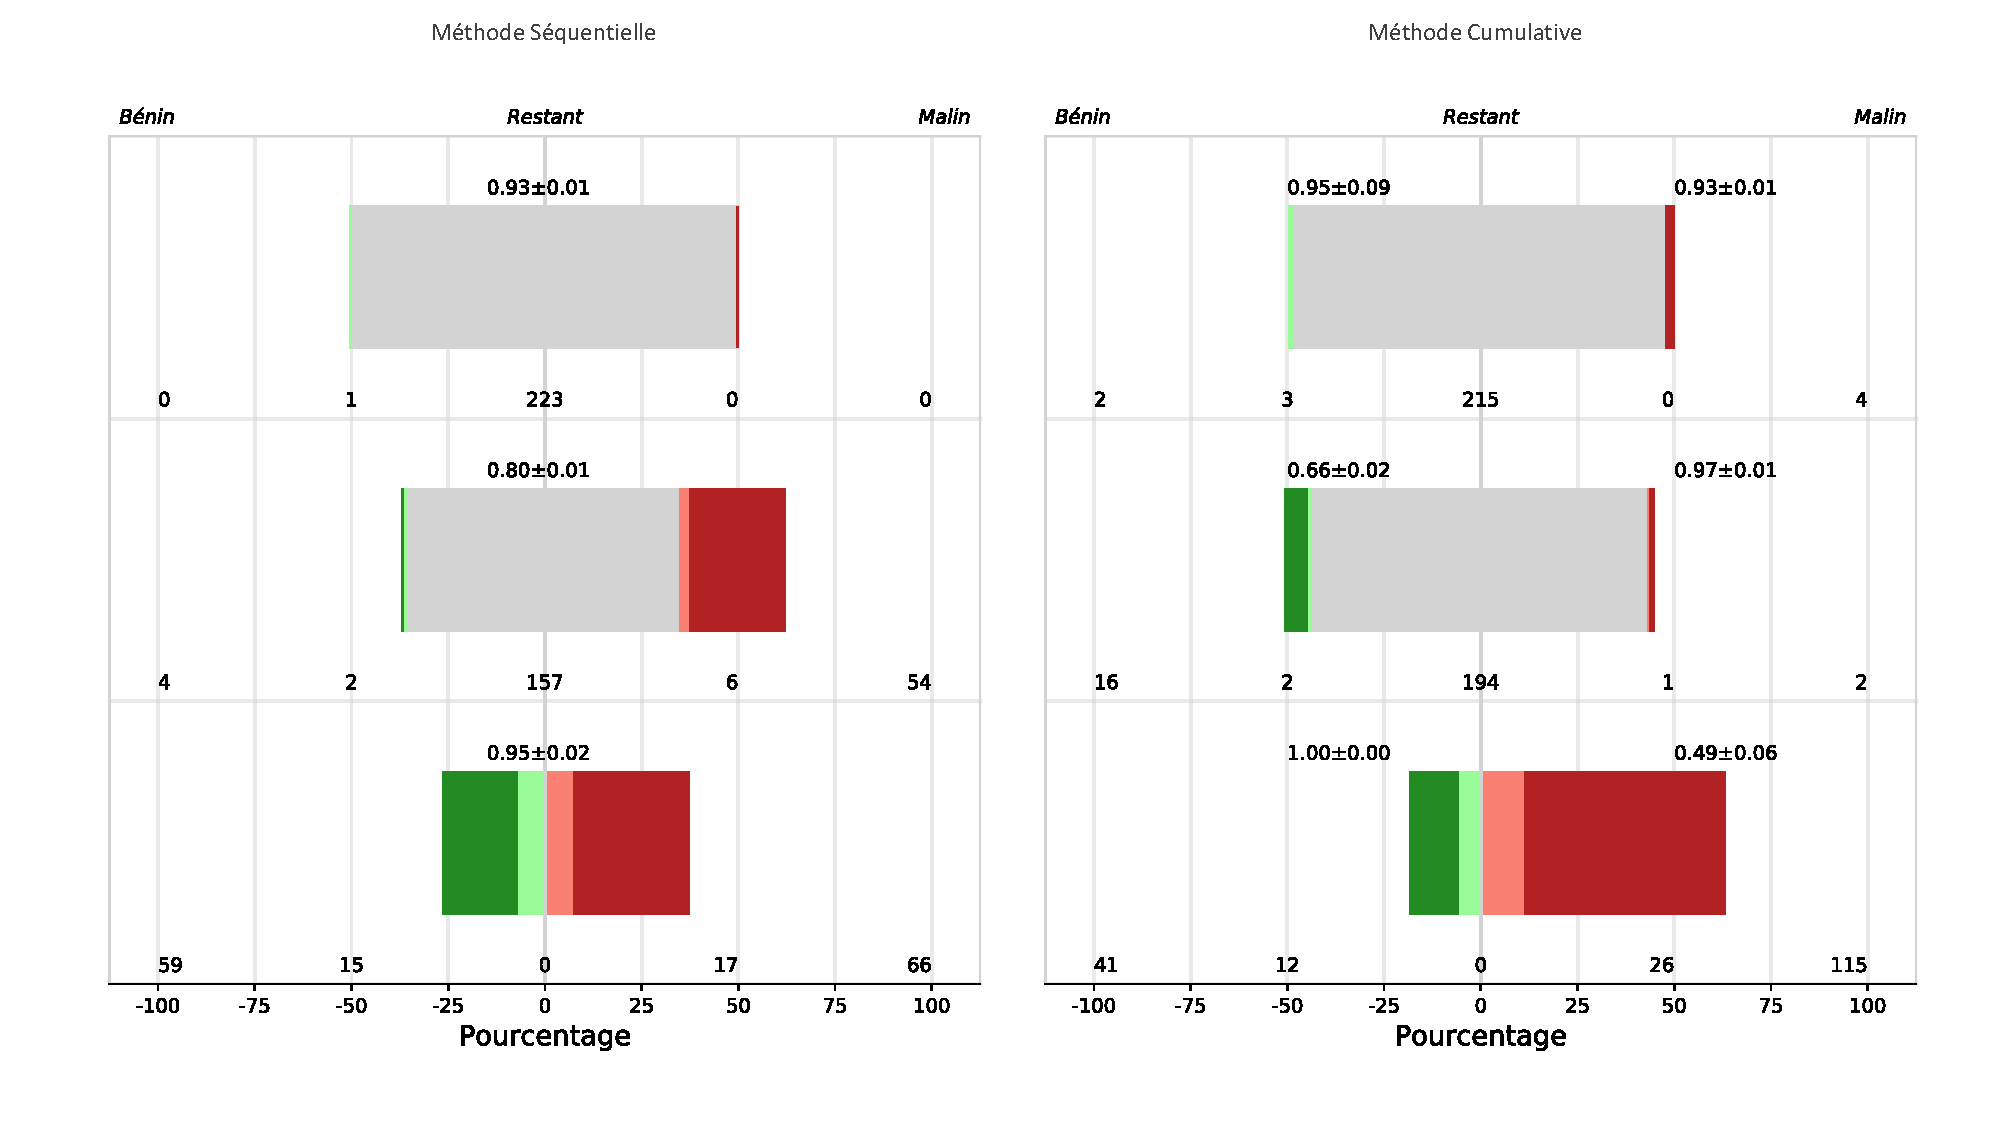
\includegraphics[width=\linewidth]{contents/chapter_8/resources/results_processus_weighted.pdf}
    \caption{}
    \label{fig:results_processus_weighted}
\end{figure}\par

\begin{figure}[H]
    \centering
    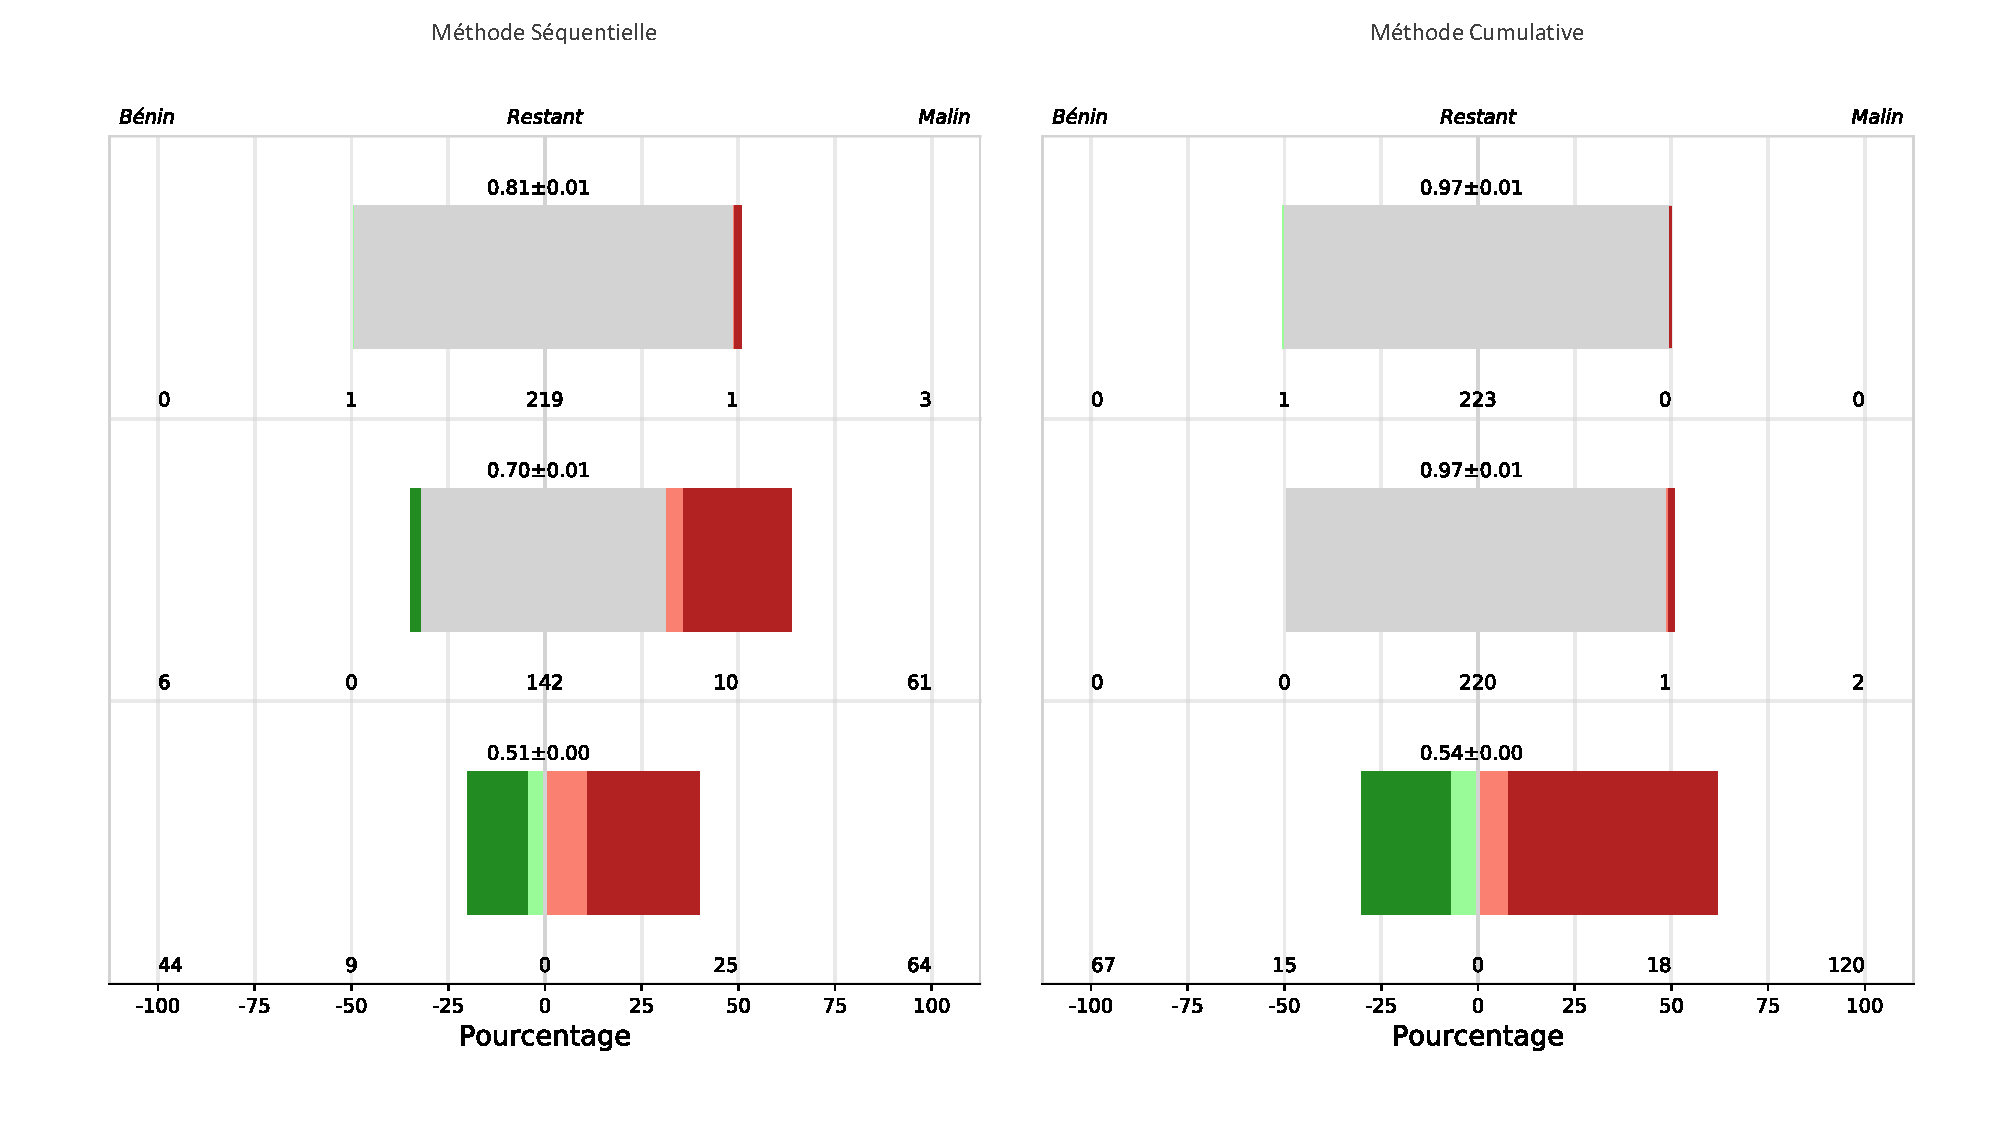
\includegraphics[width=\linewidth]{contents/chapter_8/resources/results_processus_malignant.pdf}
    \caption{}
    \label{fig:results_processus_malignant}
\end{figure}\par

\section{Discussion}